% Preamble
\documentclass[a4paper, 12pt]{article}
\usepackage[margin=1in]{geometry} % Set margin
\usepackage{pdfpages} % Insert pdf pages
\usepackage{amssymb,amsmath,amsthm, amsfonts} % Math libraries

% Custom commands
\newcommand{\sub}[1]{\subsection{\underline{#1}}}
\newcommand{\subsub}[1]{\subsubsection{\underline{#1}}}
\newcommand{\?}{\stackrel{?}{=}}
\newcommand{\R}{\ensuremath{\mathbb{R}}}
\newcommand{\F}{\ensuremath{\mathbb{F}}}
\newcommand{\eqbcuz}[1]{\text{~$\stackrel{(#1)}{=}$~}}
\renewcommand{\qed}{$$\blacksquare$$}
\renewcommand{\b}[1]{\textbf{#1}}
\renewcommand{\because}[1]{~\b{(#1)}\\}
\renewcommand{\d}{\ensuremath{\Downarrow\\~}}

% Begin Document %
\begin{document}

% Title Page
\begin{titlepage}
    %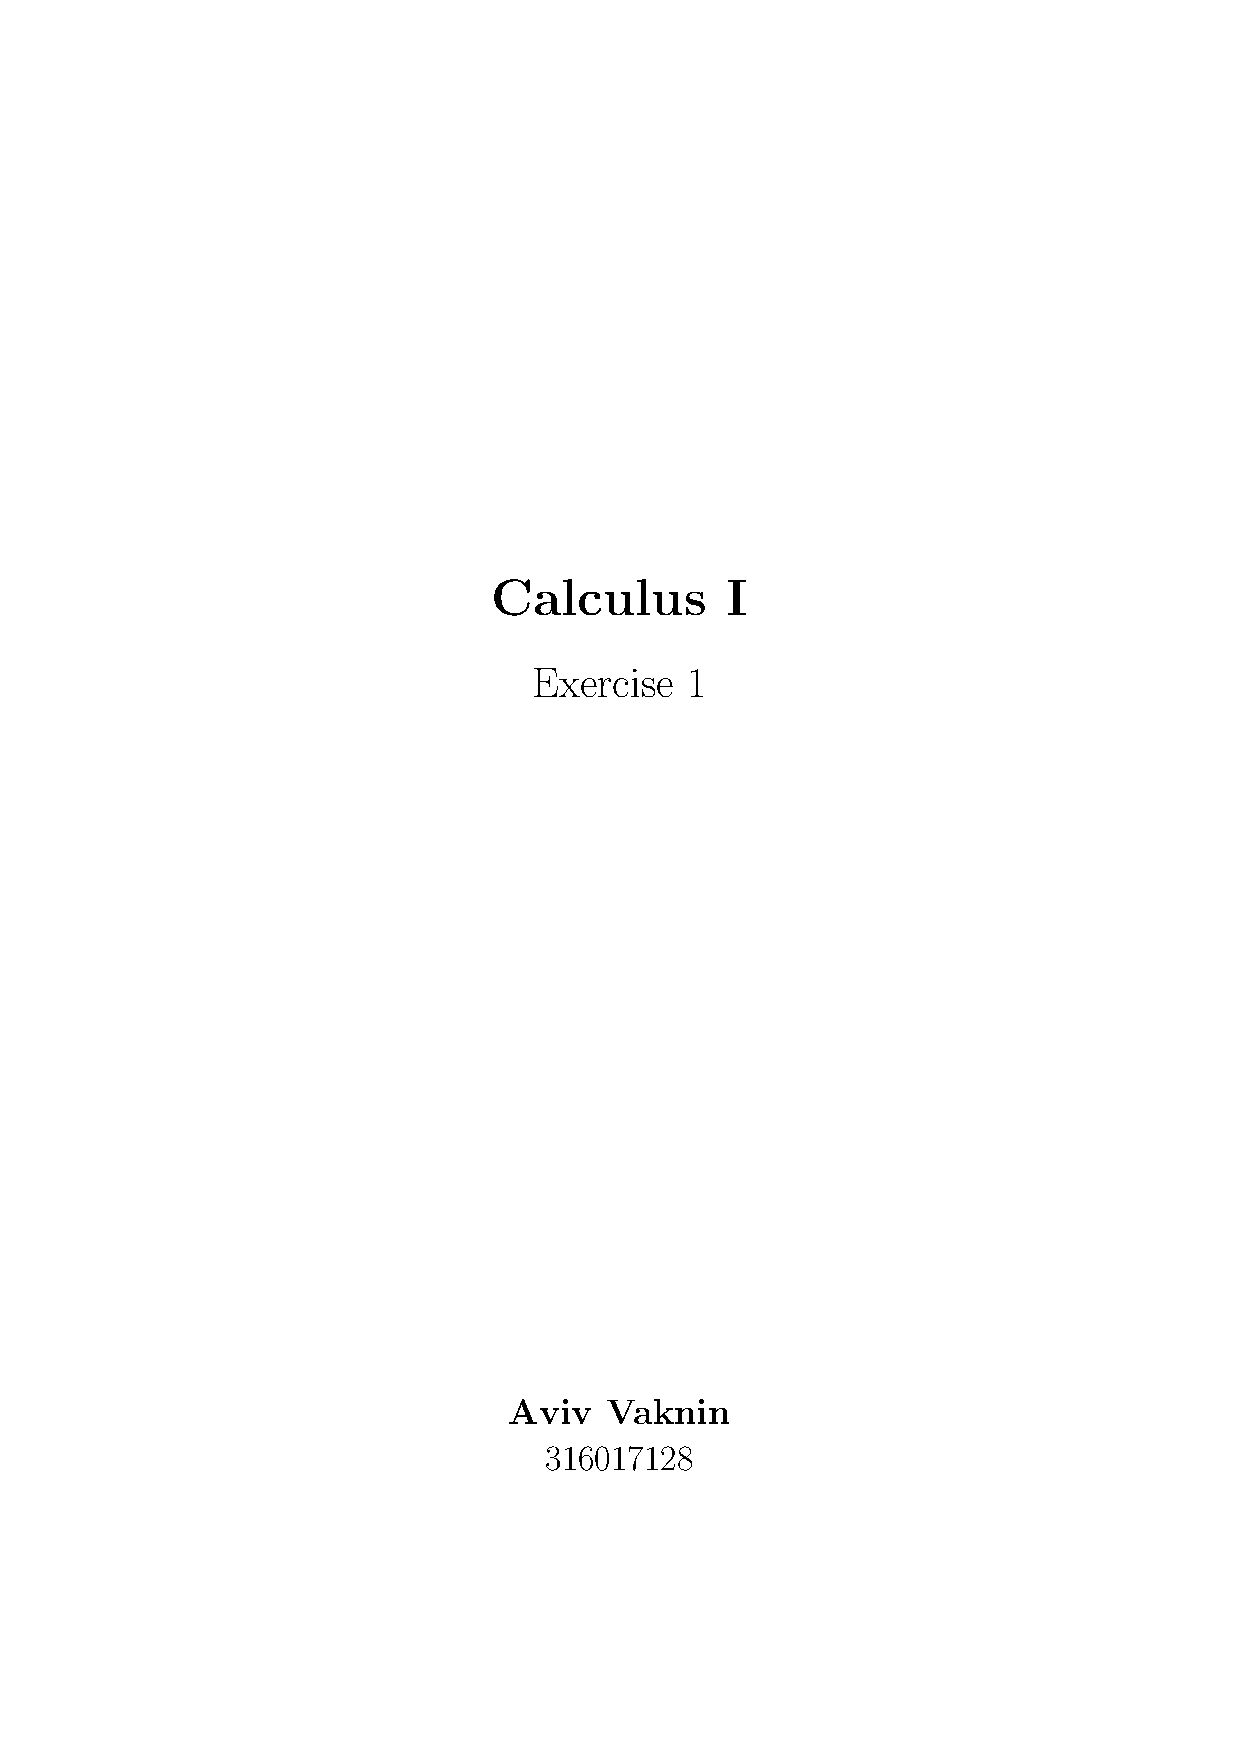
\includepdf{title.pdf}
\end{titlepage}

\section{}
\sub{}
While $i$ and $ii$ are statements, $iii$ isn't a statement,\\
because we haven't received any information about $x$'s value.
\sub{}
    \textit{i})\\
        Statement: $$ \forall{n}\in{\F} ~~ \exists{m}\in{\F} ~\big{|}~ n=m+m $$
        Negated Statement: $$ \exists{n}\in{\F} ~~ \forall{m}\in{\F} ~\big{|}~ n\neq m+m $$
    \textit{ii})\\
        Statement: $$ \forall{m,n}\in{\F} ~~ n=m+m \rightarrow -n=-m-m $$
        Negated Statement: $$ \exists{m,n}\in{\F} ~~ n=m+m ~\land~ -n\neq-m-m $$
\sub{}
    \textit{i})\\
        Statement: $$ \forall{n}\in{\F} ~~ \exists{m}\in{\F} ~\big{|}~ n=m+m $$
        Negated Statement: $$ \exists{n}\in{\F} ~~ \forall{m}\in{\F} ~\big{|}~ n\neq m+m $$

\section{}
\textit{i} is the formal representation of a field's additive inverse axiom, i.e. A4.\\
On the other hand, \textit{ii} states that in the field \F, there's a certain number, $x$,
that if we'll add it to \b{any} other number in \F, we'll receive $0_{\F}$.\\
The two statements are \b{not} logically equal.
\pagebreak

\section{}
\sub{Prove $\forall~a,b \in{\F}~ -(a-b)=(b-a)$}
First, let's find $(a-b)$'s inverse: $$ (a-b)+x=0 $$
We'll add $(b-a)$ to both sides of the equation: $$ (a-b)+(b-a)+x=(b-a) $$
And find the inverse: $$ x = (b-a) $$
Now, we can easily see that $(a-b)$ and $(b-a)$ are the inverses of each other.\\
And due to the additive inverse axiom (A4) : $$ -(a-b) = x = (b-a) $$
\qed

\sub{Prove the 'uniquness of multiplicitive inverse' property}
It is given that $ab, ac=1_{\F}$, and we need to prove that $b=c=a^{-1}$.
\subsub{$ab=1_{\F}$}
According to the multiplicitive inverse property (M4), we can deduct:
$$ b=a^{-1} $$
\subsub{$ac=1_{\F}$}
Exactly as above (M4), we can deduct:
$$ c=a^{-1} $$
Therefore, we can conclude: $$ b=c=a^{-1} $$
\qed
\pagebreak

% 4
\section{$H$ is a set that satisfies all of the field axioms,\\
$H \neq \text{\O}$, $1_H=0_H$\\
Prove that $H$ contains only a single member.}
Adding two $0_H$ should result in a $0_H$, due to axiom A3: $$ 0_H + 0_H = 0_H $$
However, because $1_H=0_H$, it also means that: $$ 1_H + 1_H = 0_H $$
Because of that, we can conculde that no other members exist in $H$, except $1_H=0_H$
\qed

% 5
\section{\F~is an ordered field, prove the following:}

%5.1
\sub{$\forall{x,y} \in{\F}~ 0_{\F}<x<y \iff 0_{\F}<y^{-1}<x^{-1} $}
\subsub{$0_{\F}<x<y ~\Longrightarrow~ 0_{\F}<y^{-1}<x^{-1} $:}
It is given that: $$ x<y $$
We'll multiple both sides of the inequality by 1, using axiom \textit{M4}: $$ xyy^{-1}<yxx^{-1} $$
It is given that $x,y > 0$ therefore we can divide the equation by $xy$: $$ y^-1 < x^-1 $$
\subsub{$0_{\F}<x<y ~\Longleftarrow~ 0_{\F}<y^{-1}<x^{-1} $:}
It is given that: $$ y^{-1}<x^{-1} $$
We'll multiple both sides of the inequality by 1, using axiom \textit{M4}: $$ y^{-1}xx^{-1}<x^{-1}yy^{-1} $$
It is given that $x^-1,y^-1 > 0$ therefore we can divide the equation by $x^-1y^-1$: $$ x<y $$
\qed\pagebreak

%5.2
\sub{$ x,y,z,w \in \F \big{|}~ x<y,~z\leq{w} ~\Longrightarrow~ x+z<y+w$}
It is given that: $$ x<y $$
We'll add $(z+w)$ to both sides, according to axiom \textit{O3}: $$ x+(z+w) < y+(z+w) $$
According to axiom \textit{A1}, we'll rearrange the inequality: $$ (x+z)+w < (y+w)+z $$
It is given that $z \leq w$, therefore if we'll remove $w$ from the left side,
and $z$ from the right side, the inequality should remain correct:
$$ x+z < y+w $$
\qed

%5.3
\sub{$ \forall{x,y} \in{\F}~ (0_{\F}<xy) \iff ((x<0_{\F} \land y<0_{\F}) \lor (0_{\F} < x \land 0_{\F}<y))  $}
\subsub{$ 0_{\F}<xy \Longrightarrow ((x<0_{\F} \land y<0_{\F}) \lor (0_{\F} < x \land 0_{\F}<y))$:}


% End
\end{document}